\documentclass[1p]{elsarticle_modified}
%\bibliographystyle{elsarticle-num}

%\usepackage[colorlinks]{hyperref}
%\usepackage{abbrmath_seonhwa} %\Abb, \Ascr, \Acal ,\Abf, \Afrak
\usepackage{amsfonts}
\usepackage{amssymb}
\usepackage{amsmath}
\usepackage{amsthm}
\usepackage{scalefnt}
\usepackage{amsbsy}
\usepackage{kotex}
\usepackage{caption}
\usepackage{subfig}
\usepackage{color}
\usepackage{graphicx}
\usepackage{xcolor} %% white, black, red, green, blue, cyan, magenta, yellow
\usepackage{float}
\usepackage{setspace}
\usepackage{hyperref}

\usepackage{tikz}
\usetikzlibrary{arrows}

\usepackage{multirow}
\usepackage{array} % fixed length table
\usepackage{hhline}

%%%%%%%%%%%%%%%%%%%%%
\makeatletter
\renewcommand*\env@matrix[1][\arraystretch]{%
	\edef\arraystretch{#1}%
	\hskip -\arraycolsep
	\let\@ifnextchar\new@ifnextchar
	\array{*\c@MaxMatrixCols c}}
\makeatother %https://tex.stackexchange.com/questions/14071/how-can-i-increase-the-line-spacing-in-a-matrix
%%%%%%%%%%%%%%%

\usepackage[normalem]{ulem}

\newcommand{\msout}[1]{\ifmmode\text{\sout{\ensuremath{#1}}}\else\sout{#1}\fi}
%SOURCE: \msout is \stkout macro in https://tex.stackexchange.com/questions/20609/strikeout-in-math-mode

\newcommand{\cancel}[1]{
	\ifmmode
	{\color{red}\msout{#1}}
	\else
	{\color{red}\sout{#1}}
	\fi
}

\newcommand{\add}[1]{
	{\color{blue}\uwave{#1}}
}

\newcommand{\replace}[2]{
	\ifmmode
	{\color{red}\msout{#1}}{\color{blue}\uwave{#2}}
	\else
	{\color{red}\sout{#1}}{\color{blue}\uwave{#2}}
	\fi
}

\newcommand{\Sol}{\mathcal{S}} %segment
\newcommand{\D}{D} %diagram
\newcommand{\A}{\mathcal{A}} %arc


%%%%%%%%%%%%%%%%%%%%%%%%%%%%%5 test

\def\sl{\operatorname{\textup{SL}}(2,\Cbb)}
\def\psl{\operatorname{\textup{PSL}}(2,\Cbb)}
\def\quan{\mkern 1mu \triangleright \mkern 1mu}

\theoremstyle{definition}
\newtheorem{thm}{Theorem}[section]
\newtheorem{prop}[thm]{Proposition}
\newtheorem{lem}[thm]{Lemma}
\newtheorem{ques}[thm]{Question}
\newtheorem{cor}[thm]{Corollary}
\newtheorem{defn}[thm]{Definition}
\newtheorem{exam}[thm]{Example}
\newtheorem{rmk}[thm]{Remark}
\newtheorem{alg}[thm]{Algorithm}

\newcommand{\I}{\sqrt{-1}}
\begin{document}

%\begin{frontmatter}
%
%\title{Boundary parabolic representations of knots up to 8 crossings}
%
%%% Group authors per affiliation:
%\author{Yunhi Cho} 
%\address{Department of Mathematics, University of Seoul, Seoul, Korea}
%\ead{yhcho@uos.ac.kr}
%
%
%\author{Seonhwa Kim} %\fnref{s_kim}}
%\address{Center for Geometry and Physics, Institute for Basic Science, Pohang, 37673, Korea}
%\ead{ryeona17@ibs.re.kr}
%
%\author{Hyuk Kim}
%\address{Department of Mathematical Sciences, Seoul National University, Seoul 08826, Korea}
%\ead{hyukkim@snu.ac.kr}
%
%\author{Seokbeom Yoon}
%\address{Department of Mathematical Sciences, Seoul National University, Seoul, 08826,  Korea}
%\ead{sbyoon15@snu.ac.kr}
%
%\begin{abstract}
%We find all boundary parabolic representation of knots up to 8 crossings.
%
%\end{abstract}
%\begin{keyword}
%    \MSC[2010] 57M25 
%\end{keyword}
%
%\end{frontmatter}

%\linenumbers
%\tableofcontents
%
\newcommand\colored[1]{\textcolor{white}{\rule[-0.35ex]{0.8em}{1.4ex}}\kern-0.8em\color{red} #1}%
%\newcommand\colored[1]{\textcolor{white}{ #1}\kern-2.17ex	\textcolor{white}{ #1}\kern-1.81ex	\textcolor{white}{ #1}\kern-2.15ex\color{red}#1	}

{\Large $\underline{12n_{0685}~(K12n_{0685})}$}

\setlength{\tabcolsep}{10pt}
\renewcommand{\arraystretch}{1.6}
\vspace{1cm}\begin{tabular}{m{100pt}>{\centering\arraybackslash}m{274pt}}
\multirow{5}{120pt}{
	\centering
	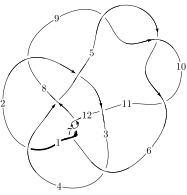
\includegraphics[width=112pt]{../../../GIT/diagram.site/Diagrams/png/2774_12n_0685.png}\\
\ \ \ A knot diagram\footnotemark}&
\allowdisplaybreaks
\textbf{Linearized knot diagam} \\
\cline{2-2}
 &
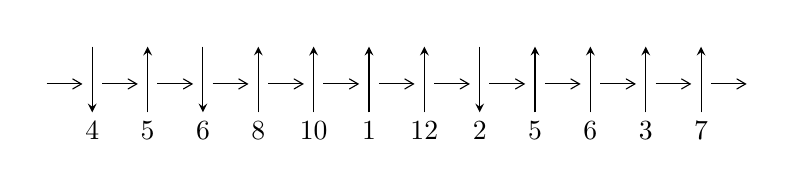
\begin{tikzpicture}[x=20pt, y=17pt]
	% nodes
	\node (C0) at (0, 0) {};
	\node (C1) at (1, 0) {};
	\node (C1U) at (1, +1) {};
	\node (C1D) at (1, -1) {4};

	\node (C2) at (2, 0) {};
	\node (C2U) at (2, +1) {};
	\node (C2D) at (2, -1) {5};

	\node (C3) at (3, 0) {};
	\node (C3U) at (3, +1) {};
	\node (C3D) at (3, -1) {6};

	\node (C4) at (4, 0) {};
	\node (C4U) at (4, +1) {};
	\node (C4D) at (4, -1) {8};

	\node (C5) at (5, 0) {};
	\node (C5U) at (5, +1) {};
	\node (C5D) at (5, -1) {10};

	\node (C6) at (6, 0) {};
	\node (C6U) at (6, +1) {};
	\node (C6D) at (6, -1) {1};

	\node (C7) at (7, 0) {};
	\node (C7U) at (7, +1) {};
	\node (C7D) at (7, -1) {12};

	\node (C8) at (8, 0) {};
	\node (C8U) at (8, +1) {};
	\node (C8D) at (8, -1) {2};

	\node (C9) at (9, 0) {};
	\node (C9U) at (9, +1) {};
	\node (C9D) at (9, -1) {5};

	\node (C10) at (10, 0) {};
	\node (C10U) at (10, +1) {};
	\node (C10D) at (10, -1) {6};

	\node (C11) at (11, 0) {};
	\node (C11U) at (11, +1) {};
	\node (C11D) at (11, -1) {3};

	\node (C12) at (12, 0) {};
	\node (C12U) at (12, +1) {};
	\node (C12D) at (12, -1) {7};
	\node (C13) at (13, 0) {};

	% arrows
	\draw[->,>={angle 60}]
	(C0) edge (C1) (C1) edge (C2) (C2) edge (C3) (C3) edge (C4) (C4) edge (C5) (C5) edge (C6) (C6) edge (C7) (C7) edge (C8) (C8) edge (C9) (C9) edge (C10) (C10) edge (C11) (C11) edge (C12) (C12) edge (C13) ;	\draw[->,>=stealth]
	(C1U) edge (C1D) (C2D) edge (C2U) (C3U) edge (C3D) (C4D) edge (C4U) (C5D) edge (C5U) (C6D) edge (C6U) (C7D) edge (C7U) (C8U) edge (C8D) (C9D) edge (C9U) (C10D) edge (C10U) (C11D) edge (C11U) (C12D) edge (C12U) ;
	\end{tikzpicture} \\
\hhline{~~} \\& 
\textbf{Solving Sequence} \\ \cline{2-2} 
 &
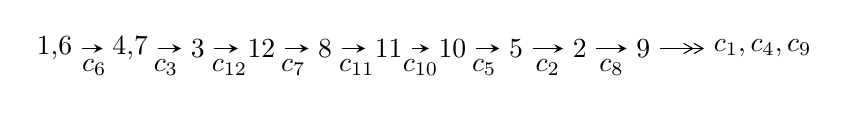
\begin{tikzpicture}[x=23pt, y=7pt]
	% node
	\node (A0) at (-1/8, 0) {1,6};
	\node (A1) at (17/16, 0) {4,7};
	\node (A2) at (17/8, 0) {3};
	\node (A3) at (25/8, 0) {12};
	\node (A4) at (33/8, 0) {8};
	\node (A5) at (41/8, 0) {11};
	\node (A6) at (49/8, 0) {10};
	\node (A7) at (57/8, 0) {5};
	\node (A8) at (65/8, 0) {2};
	\node (A9) at (73/8, 0) {9};
	\node (C1) at (1/2, -1) {$c_{6}$};
	\node (C2) at (13/8, -1) {$c_{3}$};
	\node (C3) at (21/8, -1) {$c_{12}$};
	\node (C4) at (29/8, -1) {$c_{7}$};
	\node (C5) at (37/8, -1) {$c_{11}$};
	\node (C6) at (45/8, -1) {$c_{10}$};
	\node (C7) at (53/8, -1) {$c_{5}$};
	\node (C8) at (61/8, -1) {$c_{2}$};
	\node (C9) at (69/8, -1) {$c_{8}$};
	\node (A10) at (11, 0) {$c_{1},c_{4},c_{9}$};

	% edge
	\draw[->,>=stealth]	
	(A0) edge (A1) (A1) edge (A2) (A2) edge (A3) (A3) edge (A4) (A4) edge (A5) (A5) edge (A6) (A6) edge (A7) (A7) edge (A8) (A8) edge (A9) ;
	\draw[->>,>={angle 60}]	
	(A9) edge (A10);
\end{tikzpicture} \\ 

\end{tabular} \\

\footnotetext{
The image of knot diagram is generated by the software ``\textbf{Draw programme}" developed by Andrew Bartholomew(\url{http://www.layer8.co.uk/maths/draw/index.htm\#Running-draw}), where we modified some parts for our purpose(\url{https://github.com/CATsTAILs/LinksPainter}).
}\phantom \\ \newline 
\centering \textbf{Ideals for irreducible components\footnotemark of $X_{\text{par}}$} 
 
\begin{align*}
I^u_{1}&=\langle 
-2.68320\times10^{40} u^{53}+4.36845\times10^{39} u^{52}+\cdots+1.09407\times10^{40} b-1.26785\times10^{41},\\
\phantom{I^u_{1}}&\phantom{= \langle  }1.64738\times10^{41} u^{53}-5.57914\times10^{40} u^{52}+\cdots+1.09407\times10^{40} a+4.47020\times10^{41},\;u^{54}+27 u^{52}+\cdots+12 u+1\rangle \\
I^u_{2}&=\langle 
u^{12}+u^{11}+6 u^{10}+5 u^9+13 u^8+9 u^7+10 u^6+5 u^5-3 u^4-2 u^3-6 u^2+b-2 u,\\
\phantom{I^u_{2}}&\phantom{= \langle  }- u^{12}-6 u^{10}-13 u^8-9 u^6+6 u^4- u^3+9 u^2+a-2 u,\\
\phantom{I^u_{2}}&\phantom{= \langle  }u^{15}+u^{14}+8 u^{13}+7 u^{12}+25 u^{11}+19 u^{10}+36 u^9+23 u^8+17 u^7+8 u^6-12 u^5-6 u^4-12 u^3-3 u^2+1\rangle \\
\\
\end{align*}
\raggedright * 2 irreducible components of $\dim_{\mathbb{C}}=0$, with total 69 representations.\\
\footnotetext{All coefficients of polynomials are rational numbers. But the coefficients are sometimes approximated in decimal forms when there is not enough margin.}
\newpage
\renewcommand{\arraystretch}{1}
\centering \section*{I. $I^u_{1}= \langle -2.68\times10^{40} u^{53}+4.37\times10^{39} u^{52}+\cdots+1.09\times10^{40} b-1.27\times10^{41},\;1.65\times10^{41} u^{53}-5.58\times10^{40} u^{52}+\cdots+1.09\times10^{40} a+4.47\times10^{41},\;u^{54}+27 u^{52}+\cdots+12 u+1 \rangle$}
\flushleft \textbf{(i) Arc colorings}\\
\begin{tabular}{m{7pt} m{180pt} m{7pt} m{180pt} }
\flushright $a_{1}=$&$\begin{pmatrix}0\\u\end{pmatrix}$ \\
\flushright $a_{6}=$&$\begin{pmatrix}1\\0\end{pmatrix}$ \\
\flushright $a_{4}=$&$\begin{pmatrix}-15.0573 u^{53}+5.09943 u^{52}+\cdots-402.388 u-40.8584\\2.45249 u^{53}-0.399285 u^{52}+\cdots+88.5992 u+11.5884\end{pmatrix}$ \\
\flushright $a_{7}=$&$\begin{pmatrix}1\\- u^2\end{pmatrix}$ \\
\flushright $a_{3}=$&$\begin{pmatrix}-12.6048 u^{53}+4.70015 u^{52}+\cdots-313.789 u-29.2701\\2.45249 u^{53}-0.399285 u^{52}+\cdots+88.5992 u+11.5884\end{pmatrix}$ \\
\flushright $a_{12}=$&$\begin{pmatrix}- u\\u^3+u\end{pmatrix}$ \\
\flushright $a_{8}=$&$\begin{pmatrix}u^2+1\\- u^4-2 u^2\end{pmatrix}$ \\
\flushright $a_{11}=$&$\begin{pmatrix}0.314507 u^{53}-1.02928 u^{52}+\cdots+9.85086 u+7.65563\\3.56268 u^{53}-1.46466 u^{52}+\cdots+94.5090 u+11.9366\end{pmatrix}$ \\
\flushright $a_{10}=$&$\begin{pmatrix}-3.24818 u^{53}+0.435380 u^{52}+\cdots-84.6581 u-4.28102\\3.56268 u^{53}-1.46466 u^{52}+\cdots+94.5090 u+11.9366\end{pmatrix}$ \\
\flushright $a_{5}=$&$\begin{pmatrix}-15.6451 u^{53}+5.62013 u^{52}+\cdots-401.641 u-38.9539\\2.72593 u^{53}-0.398787 u^{52}+\cdots+92.7573 u+11.9546\end{pmatrix}$ \\
\flushright $a_{2}=$&$\begin{pmatrix}-13.4990 u^{53}+5.55580 u^{52}+\cdots-340.986 u-35.3036\\5.19761 u^{53}-1.33305 u^{52}+\cdots+151.350 u+17.6227\end{pmatrix}$ \\
\flushright $a_{9}=$&$\begin{pmatrix}0.950637 u^{53}+0.741154 u^{52}+\cdots+8.38831 u+2.44017\\-3.60099 u^{53}+1.54873 u^{52}+\cdots-107.000 u-11.4663\end{pmatrix}$\\&\end{tabular}
\flushleft \textbf{(ii) Obstruction class $= -1$}\\~\\
\flushleft \textbf{(iii) Cusp Shapes $= -8.59125 u^{53}+0.873911 u^{52}+\cdots-257.258 u-36.1424$}\\~\\
\newpage\renewcommand{\arraystretch}{1}
\flushleft \textbf{(iv) u-Polynomials at the component}\newline \\
\begin{tabular}{m{50pt}|m{274pt}}
Crossings & \hspace{64pt}u-Polynomials at each crossing \\
\hline $$\begin{aligned}c_{1}\end{aligned}$$&$\begin{aligned}
&u^{54}- u^{53}+\cdots-23705 u-2291
\end{aligned}$\\
\hline $$\begin{aligned}c_{2}\end{aligned}$$&$\begin{aligned}
&u^{54}+4 u^{53}+\cdots+28 u-1
\end{aligned}$\\
\hline $$\begin{aligned}c_{3}\end{aligned}$$&$\begin{aligned}
&u^{54}- u^{53}+\cdots-2159 u+239
\end{aligned}$\\
\hline $$\begin{aligned}c_{4}\end{aligned}$$&$\begin{aligned}
&u^{54}-6 u^{52}+\cdots+22 u+1
\end{aligned}$\\
\hline $$\begin{aligned}c_{5},c_{9},c_{10}\end{aligned}$$&$\begin{aligned}
&u^{54}+u^{53}+\cdots+11 u-1
\end{aligned}$\\
\hline $$\begin{aligned}c_{6},c_{7},c_{12}\end{aligned}$$&$\begin{aligned}
&u^{54}+27 u^{52}+\cdots+12 u+1
\end{aligned}$\\
\hline $$\begin{aligned}c_{8}\end{aligned}$$&$\begin{aligned}
&u^{54}+u^{53}+\cdots+u+1
\end{aligned}$\\
\hline $$\begin{aligned}c_{11}\end{aligned}$$&$\begin{aligned}
&u^{54}-2 u^{53}+\cdots+36164 u-1709
\end{aligned}$\\
\hline
\end{tabular}\\~\\
\newpage\renewcommand{\arraystretch}{1}
\flushleft \textbf{(v) Riley Polynomials at the component}\newline \\
\begin{tabular}{m{50pt}|m{274pt}}
Crossings & \hspace{64pt}Riley Polynomials at each crossing \\
\hline $$\begin{aligned}c_{1}\end{aligned}$$&$\begin{aligned}
&y^{54}-35 y^{53}+\cdots-169277117 y+5248681
\end{aligned}$\\
\hline $$\begin{aligned}c_{2}\end{aligned}$$&$\begin{aligned}
&y^{54}+54 y^{53}+\cdots+60 y+1
\end{aligned}$\\
\hline $$\begin{aligned}c_{3}\end{aligned}$$&$\begin{aligned}
&y^{54}-53 y^{53}+\cdots+93385 y+57121
\end{aligned}$\\
\hline $$\begin{aligned}c_{4}\end{aligned}$$&$\begin{aligned}
&y^{54}-12 y^{53}+\cdots-440 y+1
\end{aligned}$\\
\hline $$\begin{aligned}c_{5},c_{9},c_{10}\end{aligned}$$&$\begin{aligned}
&y^{54}- y^{53}+\cdots-45 y+1
\end{aligned}$\\
\hline $$\begin{aligned}c_{6},c_{7},c_{12}\end{aligned}$$&$\begin{aligned}
&y^{54}+54 y^{53}+\cdots-74 y+1
\end{aligned}$\\
\hline $$\begin{aligned}c_{8}\end{aligned}$$&$\begin{aligned}
&y^{54}-49 y^{53}+\cdots-151 y+1
\end{aligned}$\\
\hline $$\begin{aligned}c_{11}\end{aligned}$$&$\begin{aligned}
&y^{54}+62 y^{53}+\cdots-555348524 y+2920681
\end{aligned}$\\
\hline
\end{tabular}\\~\\
\newpage\flushleft \textbf{(vi) Complex Volumes and Cusp Shapes}
$$\begin{array}{c|c|c}  
\text{Solutions to }I^u_{1}& \I (\text{vol} + \sqrt{-1}CS) & \text{Cusp shape}\\
 \hline 
\begin{aligned}
u &= -0.727247 + 0.655546 I \\
a &= -1.120070 - 0.569467 I \\
b &= \phantom{-}1.45756 - 0.28228 I\end{aligned}
 & -7.16637 + 5.36550 I & \phantom{-}3.29115 - 2.38015 I \\ \hline\begin{aligned}
u &= -0.727247 - 0.655546 I \\
a &= -1.120070 + 0.569467 I \\
b &= \phantom{-}1.45756 + 0.28228 I\end{aligned}
 & -7.16637 - 5.36550 I & \phantom{-}3.29115 + 2.38015 I \\ \hline\begin{aligned}
u &= -0.817874 + 0.466543 I \\
a &= -1.01459 - 1.44161 I \\
b &= \phantom{-}1.54231 + 0.48478 I\end{aligned}
 & -6.57271 - 10.55460 I & \phantom{-}4.62377 + 7.07679 I \\ \hline\begin{aligned}
u &= -0.817874 - 0.466543 I \\
a &= -1.01459 + 1.44161 I \\
b &= \phantom{-}1.54231 - 0.48478 I\end{aligned}
 & -6.57271 + 10.55460 I & \phantom{-}4.62377 - 7.07679 I \\ \hline\begin{aligned}
u &= \phantom{-}0.658331 + 0.610282 I \\
a &= \phantom{-}0.991278 - 0.834575 I \\
b &= -1.55170 + 0.23948 I\end{aligned}
 & -7.17018 + 2.76260 I & \phantom{-}2.77811 - 3.18993 I \\ \hline\begin{aligned}
u &= \phantom{-}0.658331 - 0.610282 I \\
a &= \phantom{-}0.991278 + 0.834575 I \\
b &= -1.55170 - 0.23948 I\end{aligned}
 & -7.17018 - 2.76260 I & \phantom{-}2.77811 + 3.18993 I \\ \hline\begin{aligned}
u &= \phantom{-}0.782295 + 0.434217 I \\
a &= \phantom{-}1.34381 - 1.23021 I \\
b &= -1.407260 + 0.014903 I\end{aligned}
 & -6.54490 + 2.06360 I & \phantom{-}3.73772 - 2.56730 I \\ \hline\begin{aligned}
u &= \phantom{-}0.782295 - 0.434217 I \\
a &= \phantom{-}1.34381 + 1.23021 I \\
b &= -1.407260 - 0.014903 I\end{aligned}
 & -6.54490 - 2.06360 I & \phantom{-}3.73772 + 2.56730 I \\ \hline\begin{aligned}
u &= \phantom{-}0.873178\phantom{ +0.000000I} \\
a &= -0.654136\phantom{ +0.000000I} \\
b &= \phantom{-}0.754805\phantom{ +0.000000I}\end{aligned}
 & \phantom{-}1.61182\phantom{ +0.000000I} & \phantom{-}1.21940\phantom{ +0.000000I} \\ \hline\begin{aligned}
u &= \phantom{-}0.600533 + 0.615475 I \\
a &= \phantom{-}0.088416 + 1.268790 I \\
b &= \phantom{-}0.943653 - 0.397797 I\end{aligned}
 & -0.31286 + 3.64145 I & \phantom{-}11.2572 - 9.4738 I\\
 \hline 
 \end{array}$$\newpage$$\begin{array}{c|c|c}  
\text{Solutions to }I^u_{1}& \I (\text{vol} + \sqrt{-1}CS) & \text{Cusp shape}\\
 \hline 
\begin{aligned}
u &= \phantom{-}0.600533 - 0.615475 I \\
a &= \phantom{-}0.088416 - 1.268790 I \\
b &= \phantom{-}0.943653 + 0.397797 I\end{aligned}
 & -0.31286 - 3.64145 I & \phantom{-}11.2572 + 9.4738 I \\ \hline\begin{aligned}
u &= \phantom{-}0.110651 + 1.211630 I \\
a &= \phantom{-}0.649484 + 0.213764 I \\
b &= \phantom{-}0.742245 + 0.814719 I\end{aligned}
 & -2.38520 + 2.82306 I & \phantom{-0.000000 } 0 \\ \hline\begin{aligned}
u &= \phantom{-}0.110651 - 1.211630 I \\
a &= \phantom{-}0.649484 - 0.213764 I \\
b &= \phantom{-}0.742245 - 0.814719 I\end{aligned}
 & -2.38520 - 2.82306 I & \phantom{-0.000000 } 0 \\ \hline\begin{aligned}
u &= -0.142943 + 1.223340 I \\
a &= \phantom{-}0.983994 - 0.047102 I \\
b &= -0.904696 + 0.730444 I\end{aligned}
 & -4.86587 + 0.83794 I & \phantom{-0.000000 } 0 \\ \hline\begin{aligned}
u &= -0.142943 - 1.223340 I \\
a &= \phantom{-}0.983994 + 0.047102 I \\
b &= -0.904696 - 0.730444 I\end{aligned}
 & -4.86587 - 0.83794 I & \phantom{-0.000000 } 0 \\ \hline\begin{aligned}
u &= -0.722991\phantom{ +0.000000I} \\
a &= -1.44649\phantom{ +0.000000I} \\
b &= \phantom{-}0.416019\phantom{ +0.000000I}\end{aligned}
 & \phantom{-}5.96932\phantom{ +0.000000I} & \phantom{-}18.1570\phantom{ +0.000000I} \\ \hline\begin{aligned}
u &= -0.591356 + 0.394727 I \\
a &= \phantom{-}1.15354 + 1.47575 I \\
b &= -1.372070 - 0.284950 I\end{aligned}
 & -2.42244 - 1.86344 I & \phantom{-}0.32896 + 2.97816 I \\ \hline\begin{aligned}
u &= -0.591356 - 0.394727 I \\
a &= \phantom{-}1.15354 - 1.47575 I \\
b &= -1.372070 + 0.284950 I\end{aligned}
 & -2.42244 + 1.86344 I & \phantom{-}0.32896 - 2.97816 I \\ \hline\begin{aligned}
u &= -0.284927 + 1.273200 I \\
a &= -0.610811 - 0.705027 I \\
b &= \phantom{-}0.378777 + 0.245213 I\end{aligned}
 & \phantom{-}2.02546 - 3.64647 I & \phantom{-0.000000 } 0 \\ \hline\begin{aligned}
u &= -0.284927 - 1.273200 I \\
a &= -0.610811 + 0.705027 I \\
b &= \phantom{-}0.378777 - 0.245213 I\end{aligned}
 & \phantom{-}2.02546 + 3.64647 I & \phantom{-0.000000 } 0\\
 \hline 
 \end{array}$$\newpage$$\begin{array}{c|c|c}  
\text{Solutions to }I^u_{1}& \I (\text{vol} + \sqrt{-1}CS) & \text{Cusp shape}\\
 \hline 
\begin{aligned}
u &= \phantom{-}0.425694 + 1.274300 I \\
a &= -0.137225 + 0.299114 I \\
b &= \phantom{-}0.804888 + 0.001080 I\end{aligned}
 & -2.34924 + 4.63206 I & \phantom{-0.000000 } 0 \\ \hline\begin{aligned}
u &= \phantom{-}0.425694 - 1.274300 I \\
a &= -0.137225 - 0.299114 I \\
b &= \phantom{-}0.804888 - 0.001080 I\end{aligned}
 & -2.34924 - 4.63206 I & \phantom{-0.000000 } 0 \\ \hline\begin{aligned}
u &= \phantom{-}0.079610 + 1.366620 I \\
a &= \phantom{-}0.059053 - 0.444591 I \\
b &= -0.069313 + 0.938702 I\end{aligned}
 & -3.77402 + 1.92762 I & \phantom{-0.000000 } 0 \\ \hline\begin{aligned}
u &= \phantom{-}0.079610 - 1.366620 I \\
a &= \phantom{-}0.059053 + 0.444591 I \\
b &= -0.069313 - 0.938702 I\end{aligned}
 & -3.77402 - 1.92762 I & \phantom{-0.000000 } 0 \\ \hline\begin{aligned}
u &= \phantom{-}0.630083\phantom{ +0.000000I} \\
a &= -0.310787\phantom{ +0.000000I} \\
b &= \phantom{-}0.798544\phantom{ +0.000000I}\end{aligned}
 & \phantom{-}1.05920\phantom{ +0.000000I} & \phantom{-}8.70240\phantom{ +0.000000I} \\ \hline\begin{aligned}
u &= -0.027362 + 1.385500 I \\
a &= \phantom{-}0.562065 + 0.539030 I \\
b &= \phantom{-}1.62034 - 0.54932 I\end{aligned}
 & -1.87045 - 0.53073 I & \phantom{-0.000000 } 0 \\ \hline\begin{aligned}
u &= -0.027362 - 1.385500 I \\
a &= \phantom{-}0.562065 - 0.539030 I \\
b &= \phantom{-}1.62034 + 0.54932 I\end{aligned}
 & -1.87045 + 0.53073 I & \phantom{-0.000000 } 0 \\ \hline\begin{aligned}
u &= -0.057418 + 1.395130 I \\
a &= -1.54371 + 0.64324 I \\
b &= -1.136840 - 0.424786 I\end{aligned}
 & -5.83103 - 3.79502 I & \phantom{-0.000000 } 0 \\ \hline\begin{aligned}
u &= -0.057418 - 1.395130 I \\
a &= -1.54371 - 0.64324 I \\
b &= -1.136840 + 0.424786 I\end{aligned}
 & -5.83103 + 3.79502 I & \phantom{-0.000000 } 0 \\ \hline\begin{aligned}
u &= -0.16335 + 1.41281 I \\
a &= -0.556055 + 0.832668 I \\
b &= -0.72716 - 1.67965 I\end{aligned}
 & -5.98732 - 6.70530 I & \phantom{-0.000000 } 0\\
 \hline 
 \end{array}$$\newpage$$\begin{array}{c|c|c}  
\text{Solutions to }I^u_{1}& \I (\text{vol} + \sqrt{-1}CS) & \text{Cusp shape}\\
 \hline 
\begin{aligned}
u &= -0.16335 - 1.41281 I \\
a &= -0.556055 - 0.832668 I \\
b &= -0.72716 + 1.67965 I\end{aligned}
 & -5.98732 + 6.70530 I & \phantom{-0.000000 } 0 \\ \hline\begin{aligned}
u &= -0.493438 + 0.257877 I \\
a &= \phantom{-}0.35961 + 2.32754 I \\
b &= -0.373419 - 1.315190 I\end{aligned}
 & -0.60246 - 4.33501 I & \phantom{-}8.99729 + 10.44789 I \\ \hline\begin{aligned}
u &= -0.493438 - 0.257877 I \\
a &= \phantom{-}0.35961 - 2.32754 I \\
b &= -0.373419 + 1.315190 I\end{aligned}
 & -0.60246 + 4.33501 I & \phantom{-}8.99729 - 10.44789 I \\ \hline\begin{aligned}
u &= \phantom{-}0.509006 + 0.161109 I \\
a &= -0.289495 - 0.461991 I \\
b &= \phantom{-}0.494322 + 0.360163 I\end{aligned}
 & \phantom{-}0.947117 + 0.129909 I & \phantom{-}11.27686 - 2.22644 I \\ \hline\begin{aligned}
u &= \phantom{-}0.509006 - 0.161109 I \\
a &= -0.289495 + 0.461991 I \\
b &= \phantom{-}0.494322 - 0.360163 I\end{aligned}
 & \phantom{-}0.947117 - 0.129909 I & \phantom{-}11.27686 + 2.22644 I \\ \hline\begin{aligned}
u &= -0.22783 + 1.45064 I \\
a &= -0.329271 + 1.292780 I \\
b &= -1.72420 - 0.54667 I\end{aligned}
 & -8.34733 - 4.89875 I & \phantom{-0.000000 } 0 \\ \hline\begin{aligned}
u &= -0.22783 - 1.45064 I \\
a &= -0.329271 - 1.292780 I \\
b &= -1.72420 + 0.54667 I\end{aligned}
 & -8.34733 + 4.89875 I & \phantom{-0.000000 } 0 \\ \hline\begin{aligned}
u &= \phantom{-}0.07299 + 1.48329 I \\
a &= \phantom{-}0.151391 + 1.225570 I \\
b &= -0.143907 - 0.422731 I\end{aligned}
 & -8.28129 + 3.22679 I & \phantom{-0.000000 } 0 \\ \hline\begin{aligned}
u &= \phantom{-}0.07299 - 1.48329 I \\
a &= \phantom{-}0.151391 - 1.225570 I \\
b &= -0.143907 + 0.422731 I\end{aligned}
 & -8.28129 - 3.22679 I & \phantom{-0.000000 } 0 \\ \hline\begin{aligned}
u &= \phantom{-}0.069990 + 0.509753 I \\
a &= \phantom{-}1.19972 + 2.08736 I \\
b &= -0.070424 + 0.287433 I\end{aligned}
 & -1.81357 + 2.38364 I & \phantom{-}0.95087 - 1.41179 I\\
 \hline 
 \end{array}$$\newpage$$\begin{array}{c|c|c}  
\text{Solutions to }I^u_{1}& \I (\text{vol} + \sqrt{-1}CS) & \text{Cusp shape}\\
 \hline 
\begin{aligned}
u &= \phantom{-}0.069990 - 0.509753 I \\
a &= \phantom{-}1.19972 - 2.08736 I \\
b &= -0.070424 - 0.287433 I\end{aligned}
 & -1.81357 - 2.38364 I & \phantom{-}0.95087 + 1.41179 I \\ \hline\begin{aligned}
u &= \phantom{-}0.29461 + 1.50032 I \\
a &= -0.017831 - 1.339470 I \\
b &= -1.42401 + 0.25866 I\end{aligned}
 & -12.8030 + 6.0112 I & \phantom{-0.000000 } 0 \\ \hline\begin{aligned}
u &= \phantom{-}0.29461 - 1.50032 I \\
a &= -0.017831 + 1.339470 I \\
b &= -1.42401 - 0.25866 I\end{aligned}
 & -12.8030 - 6.0112 I & \phantom{-0.000000 } 0 \\ \hline\begin{aligned}
u &= -0.30047 + 1.51505 I \\
a &= \phantom{-}0.318429 - 1.306700 I \\
b &= \phantom{-}1.68707 + 0.60140 I\end{aligned}
 & -12.9927 - 14.6415 I & \phantom{-0.000000 } 0 \\ \hline\begin{aligned}
u &= -0.30047 - 1.51505 I \\
a &= \phantom{-}0.318429 + 1.306700 I \\
b &= \phantom{-}1.68707 - 0.60140 I\end{aligned}
 & -12.9927 + 14.6415 I & \phantom{-0.000000 } 0 \\ \hline\begin{aligned}
u &= \phantom{-}0.20551 + 1.53545 I \\
a &= -0.261245 - 0.741640 I \\
b &= -1.86481 + 0.32365 I\end{aligned}
 & -14.2076 + 5.8827 I & \phantom{-0.000000 } 0 \\ \hline\begin{aligned}
u &= \phantom{-}0.20551 - 1.53545 I \\
a &= -0.261245 + 0.741640 I \\
b &= -1.86481 - 0.32365 I\end{aligned}
 & -14.2076 - 5.8827 I & \phantom{-0.000000 } 0 \\ \hline\begin{aligned}
u &= \phantom{-}0.22302 + 1.54513 I \\
a &= \phantom{-}0.600789 + 0.941334 I \\
b &= \phantom{-}1.199140 - 0.475695 I\end{aligned}
 & -7.40823 + 6.78161 I & \phantom{-0.000000 } 0 \\ \hline\begin{aligned}
u &= \phantom{-}0.22302 - 1.54513 I \\
a &= \phantom{-}0.600789 - 0.941334 I \\
b &= \phantom{-}1.199140 + 0.475695 I\end{aligned}
 & -7.40823 - 6.78161 I & \phantom{-0.000000 } 0 \\ \hline\begin{aligned}
u &= -0.20084 + 1.57551 I \\
a &= \phantom{-}0.122450 - 0.759219 I \\
b &= \phantom{-}1.53708 - 0.00469 I\end{aligned}
 & -14.6210 + 2.0031 I & \phantom{-0.000000 } 0\\
 \hline 
 \end{array}$$\newpage$$\begin{array}{c|c|c}  
\text{Solutions to }I^u_{1}& \I (\text{vol} + \sqrt{-1}CS) & \text{Cusp shape}\\
 \hline 
\begin{aligned}
u &= -0.20084 - 1.57551 I \\
a &= \phantom{-}0.122450 + 0.759219 I \\
b &= \phantom{-}1.53708 + 0.00469 I\end{aligned}
 & -14.6210 - 2.0031 I & \phantom{-0.000000 } 0 \\ \hline\begin{aligned}
u &= -0.320973 + 0.010257 I \\
a &= \phantom{-}1.47897 + 4.46204 I \\
b &= -0.824971 - 0.660602 I\end{aligned}
 & -1.13474 - 2.72736 I & \phantom{-}9.52970 + 1.05898 I \\ \hline\begin{aligned}
u &= -0.320973 - 0.010257 I \\
a &= \phantom{-}1.47897 - 4.46204 I \\
b &= -0.824971 + 0.660602 I\end{aligned}
 & -1.13474 + 2.72736 I & \phantom{-}9.52970 - 1.05898 I \\ \hline\begin{aligned}
u &= -0.132701\phantom{ +0.000000I} \\
a &= \phantom{-}4.04601\phantom{ +0.000000I} \\
b &= \phantom{-}1.40543\phantom{ +0.000000I}\end{aligned}
 & \phantom{-}2.79911\phantom{ +0.000000I} & -5.45500\phantom{ +0.000000I}\\
 \hline 
 \end{array}$$\newpage\newpage\renewcommand{\arraystretch}{1}
\centering \section*{II. $I^u_{2}= \langle u^{12}+u^{11}+\cdots+b-2 u,\;- u^{12}-6 u^{10}+\cdots+a-2 u,\;u^{15}+u^{14}+\cdots-3 u^2+1 \rangle$}
\flushleft \textbf{(i) Arc colorings}\\
\begin{tabular}{m{7pt} m{180pt} m{7pt} m{180pt} }
\flushright $a_{1}=$&$\begin{pmatrix}0\\u\end{pmatrix}$ \\
\flushright $a_{6}=$&$\begin{pmatrix}1\\0\end{pmatrix}$ \\
\flushright $a_{4}=$&$\begin{pmatrix}u^{12}+6 u^{10}+13 u^8+9 u^6-6 u^4+u^3-9 u^2+2 u\\- u^{12}- u^{11}+\cdots+6 u^2+2 u\end{pmatrix}$ \\
\flushright $a_{7}=$&$\begin{pmatrix}1\\- u^2\end{pmatrix}$ \\
\flushright $a_{3}=$&$\begin{pmatrix}- u^{11}-5 u^9-9 u^7- u^6-5 u^5-3 u^4+3 u^3-3 u^2+4 u\\- u^{12}- u^{11}+\cdots+6 u^2+2 u\end{pmatrix}$ \\
\flushright $a_{12}=$&$\begin{pmatrix}- u\\u^3+u\end{pmatrix}$ \\
\flushright $a_{8}=$&$\begin{pmatrix}u^2+1\\- u^4-2 u^2\end{pmatrix}$ \\
\flushright $a_{11}=$&$\begin{pmatrix}- u^{13}-2 u^{12}+\cdots+u-3\\- u^{13}- u^{12}+\cdots-2 u-1\end{pmatrix}$ \\
\flushright $a_{10}=$&$\begin{pmatrix}- u^{12}- u^{11}+\cdots+3 u-2\\- u^{13}- u^{12}+\cdots-2 u-1\end{pmatrix}$ \\
\flushright $a_{5}=$&$\begin{pmatrix}- u^{11}-5 u^9-9 u^7-2 u^6-6 u^5-6 u^4+u^3-5 u^2+3 u+1\\u^{14}+u^{13}+\cdots+4 u^2+2 u\end{pmatrix}$ \\
\flushright $a_{2}=$&$\begin{pmatrix}-2 u^{14}-3 u^{13}+\cdots+5 u-3\\2 u^{13}+u^{12}+\cdots+u^2+1\end{pmatrix}$ \\
\flushright $a_{9}=$&$\begin{pmatrix}u^{13}- u^{12}+\cdots+6 u-2\\-2 u^{13}-2 u^{12}+\cdots- u-1\end{pmatrix}$\\&\end{tabular}
\flushleft \textbf{(ii) Obstruction class $= 1$}\\~\\
\flushleft \textbf{(iii) Cusp Shapes $= -7 u^{13}-6 u^{12}-49 u^{11}-38 u^{10}-130 u^9-90 u^8-150 u^7-87 u^6-39 u^5-10 u^4+58 u^3+27 u^2+31 u+8$}\\~\\
\newpage\renewcommand{\arraystretch}{1}
\flushleft \textbf{(iv) u-Polynomials at the component}\newline \\
\begin{tabular}{m{50pt}|m{274pt}}
Crossings & \hspace{64pt}u-Polynomials at each crossing \\
\hline $$\begin{aligned}c_{1}\end{aligned}$$&$\begin{aligned}
&u^{15}-12 u^{14}+\cdots+15 u-1
\end{aligned}$\\
\hline $$\begin{aligned}c_{2}\end{aligned}$$&$\begin{aligned}
&u^{15}+3 u^{14}+\cdots+4 u^2-1
\end{aligned}$\\
\hline $$\begin{aligned}c_{3}\end{aligned}$$&$\begin{aligned}
&u^{15}-6 u^{13}+\cdots+3 u-1
\end{aligned}$\\
\hline $$\begin{aligned}c_{4}\end{aligned}$$&$\begin{aligned}
&u^{15}- u^{14}+\cdots-6 u^2+1
\end{aligned}$\\
\hline $$\begin{aligned}c_{5}\end{aligned}$$&$\begin{aligned}
&u^{15}-4 u^{13}+\cdots+u-1
\end{aligned}$\\
\hline $$\begin{aligned}c_{6},c_{7}\end{aligned}$$&$\begin{aligned}
&u^{15}+u^{14}+\cdots-3 u^2+1
\end{aligned}$\\
\hline $$\begin{aligned}c_{8}\end{aligned}$$&$\begin{aligned}
&u^{15}-6 u^{13}+\cdots- u-1
\end{aligned}$\\
\hline $$\begin{aligned}c_{9},c_{10}\end{aligned}$$&$\begin{aligned}
&u^{15}-4 u^{13}+\cdots+u+1
\end{aligned}$\\
\hline $$\begin{aligned}c_{11}\end{aligned}$$&$\begin{aligned}
&u^{15}- u^{14}+\cdots+4 u^2-1
\end{aligned}$\\
\hline $$\begin{aligned}c_{12}\end{aligned}$$&$\begin{aligned}
&u^{15}- u^{14}+\cdots+3 u^2-1
\end{aligned}$\\
\hline
\end{tabular}\\~\\
\newpage\renewcommand{\arraystretch}{1}
\flushleft \textbf{(v) Riley Polynomials at the component}\newline \\
\begin{tabular}{m{50pt}|m{274pt}}
Crossings & \hspace{64pt}Riley Polynomials at each crossing \\
\hline $$\begin{aligned}c_{1}\end{aligned}$$&$\begin{aligned}
&y^{15}-2 y^{14}+\cdots+49 y-1
\end{aligned}$\\
\hline $$\begin{aligned}c_{2}\end{aligned}$$&$\begin{aligned}
&y^{15}+7 y^{14}+\cdots+8 y-1
\end{aligned}$\\
\hline $$\begin{aligned}c_{3}\end{aligned}$$&$\begin{aligned}
&y^{15}-12 y^{14}+\cdots+11 y-1
\end{aligned}$\\
\hline $$\begin{aligned}c_{4}\end{aligned}$$&$\begin{aligned}
&y^{15}-15 y^{14}+\cdots+12 y-1
\end{aligned}$\\
\hline $$\begin{aligned}c_{5},c_{9},c_{10}\end{aligned}$$&$\begin{aligned}
&y^{15}-8 y^{14}+\cdots-3 y-1
\end{aligned}$\\
\hline $$\begin{aligned}c_{6},c_{7},c_{12}\end{aligned}$$&$\begin{aligned}
&y^{15}+15 y^{14}+\cdots+6 y-1
\end{aligned}$\\
\hline $$\begin{aligned}c_{8}\end{aligned}$$&$\begin{aligned}
&y^{15}-12 y^{14}+\cdots+15 y-1
\end{aligned}$\\
\hline $$\begin{aligned}c_{11}\end{aligned}$$&$\begin{aligned}
&y^{15}+3 y^{14}+\cdots+8 y-1
\end{aligned}$\\
\hline
\end{tabular}\\~\\
\newpage\flushleft \textbf{(vi) Complex Volumes and Cusp Shapes}
$$\begin{array}{c|c|c}  
\text{Solutions to }I^u_{2}& \I (\text{vol} + \sqrt{-1}CS) & \text{Cusp shape}\\
 \hline 
\begin{aligned}
u &= -0.917074\phantom{ +0.000000I} \\
a &= \phantom{-}0.317754\phantom{ +0.000000I} \\
b &= -0.706611\phantom{ +0.000000I}\end{aligned}
 & \phantom{-}2.01181\phantom{ +0.000000I} & \phantom{-}23.5320\phantom{ +0.000000I} \\ \hline\begin{aligned}
u &= -0.074215 + 1.225200 I \\
a &= \phantom{-}1.37536 + 0.51706 I \\
b &= -0.477263 + 0.644746 I\end{aligned}
 & -4.31514 + 2.06106 I & \phantom{-}2.80971 - 3.49368 I \\ \hline\begin{aligned}
u &= -0.074215 - 1.225200 I \\
a &= \phantom{-}1.37536 - 0.51706 I \\
b &= -0.477263 - 0.644746 I\end{aligned}
 & -4.31514 - 2.06106 I & \phantom{-}2.80971 + 3.49368 I \\ \hline\begin{aligned}
u &= \phantom{-}0.738441\phantom{ +0.000000I} \\
a &= -1.88795\phantom{ +0.000000I} \\
b &= \phantom{-}0.822162\phantom{ +0.000000I}\end{aligned}
 & \phantom{-}5.31354\phantom{ +0.000000I} & \phantom{-}5.05140\phantom{ +0.000000I} \\ \hline\begin{aligned}
u &= -0.391682 + 1.206530 I \\
a &= -0.448299 + 0.314891 I \\
b &= -0.633852 - 0.204044 I\end{aligned}
 & -1.63448 - 4.71343 I & \phantom{-}9.81376 + 7.25544 I \\ \hline\begin{aligned}
u &= -0.391682 - 1.206530 I \\
a &= -0.448299 - 0.314891 I \\
b &= -0.633852 + 0.204044 I\end{aligned}
 & -1.63448 + 4.71343 I & \phantom{-}9.81376 - 7.25544 I \\ \hline\begin{aligned}
u &= \phantom{-}0.310878 + 1.284290 I \\
a &= -0.579681 + 0.974594 I \\
b &= \phantom{-}0.784151 - 0.173085 I\end{aligned}
 & \phantom{-}1.30709 + 3.78442 I & \phantom{-}1.00032 - 4.22940 I \\ \hline\begin{aligned}
u &= \phantom{-}0.310878 - 1.284290 I \\
a &= -0.579681 - 0.974594 I \\
b &= \phantom{-}0.784151 + 0.173085 I\end{aligned}
 & \phantom{-}1.30709 - 3.78442 I & \phantom{-}1.00032 + 4.22940 I \\ \hline\begin{aligned}
u &= \phantom{-}0.117562 + 1.341930 I \\
a &= \phantom{-}0.493543 + 0.042097 I \\
b &= \phantom{-}1.57940 + 0.48851 I\end{aligned}
 & -1.30643 + 1.67719 I & \phantom{-}7.37794 - 3.24911 I \\ \hline\begin{aligned}
u &= \phantom{-}0.117562 - 1.341930 I \\
a &= \phantom{-}0.493543 - 0.042097 I \\
b &= \phantom{-}1.57940 - 0.48851 I\end{aligned}
 & -1.30643 - 1.67719 I & \phantom{-}7.37794 + 3.24911 I\\
 \hline 
 \end{array}$$\newpage$$\begin{array}{c|c|c}  
\text{Solutions to }I^u_{2}& \I (\text{vol} + \sqrt{-1}CS) & \text{Cusp shape}\\
 \hline 
\begin{aligned}
u &= -0.19173 + 1.46876 I \\
a &= -0.602052 + 1.218750 I \\
b &= -1.25573 - 0.76427 I\end{aligned}
 & -7.60875 - 5.65349 I & \phantom{-}0.73377 + 5.33315 I \\ \hline\begin{aligned}
u &= -0.19173 - 1.46876 I \\
a &= -0.602052 - 1.218750 I \\
b &= -1.25573 + 0.76427 I\end{aligned}
 & -7.60875 + 5.65349 I & \phantom{-}0.73377 - 5.33315 I \\ \hline\begin{aligned}
u &= -0.356463 + 0.351194 I \\
a &= -0.23894 + 3.19582 I \\
b &= -0.810143 - 0.625914 I\end{aligned}
 & -1.51467 - 3.34740 I & \phantom{-}2.47459 + 9.57162 I \\ \hline\begin{aligned}
u &= -0.356463 - 0.351194 I \\
a &= -0.23894 - 3.19582 I \\
b &= -0.810143 + 0.625914 I\end{aligned}
 & -1.51467 + 3.34740 I & \phantom{-}2.47459 - 9.57162 I \\ \hline\begin{aligned}
u &= \phantom{-}0.349922\phantom{ +0.000000I} \\
a &= -0.429663\phantom{ +0.000000I} \\
b &= \phantom{-}1.51132\phantom{ +0.000000I}\end{aligned}
 & \phantom{-}3.08020\phantom{ +0.000000I} & \phantom{-}23.9960\phantom{ +0.000000I}\\
 \hline 
 \end{array}$$\newpage
\newpage\renewcommand{\arraystretch}{1}
\centering \section*{ III. u-Polynomials}
\begin{tabular}{m{50pt}|m{274pt}}
Crossings & \hspace{64pt}u-Polynomials at each crossing \\
\hline $$\begin{aligned}c_{1}\end{aligned}$$&$\begin{aligned}
&(u^{15}-12 u^{14}+\cdots+15 u-1)(u^{54}- u^{53}+\cdots-23705 u-2291)
\end{aligned}$\\
\hline $$\begin{aligned}c_{2}\end{aligned}$$&$\begin{aligned}
&(u^{15}+3 u^{14}+\cdots+4 u^2-1)(u^{54}+4 u^{53}+\cdots+28 u-1)
\end{aligned}$\\
\hline $$\begin{aligned}c_{3}\end{aligned}$$&$\begin{aligned}
&(u^{15}-6 u^{13}+\cdots+3 u-1)(u^{54}- u^{53}+\cdots-2159 u+239)
\end{aligned}$\\
\hline $$\begin{aligned}c_{4}\end{aligned}$$&$\begin{aligned}
&(u^{15}- u^{14}+\cdots-6 u^2+1)(u^{54}-6 u^{52}+\cdots+22 u+1)
\end{aligned}$\\
\hline $$\begin{aligned}c_{5}\end{aligned}$$&$\begin{aligned}
&(u^{15}-4 u^{13}+\cdots+u-1)(u^{54}+u^{53}+\cdots+11 u-1)
\end{aligned}$\\
\hline $$\begin{aligned}c_{6},c_{7}\end{aligned}$$&$\begin{aligned}
&(u^{15}+u^{14}+\cdots-3 u^2+1)(u^{54}+27 u^{52}+\cdots+12 u+1)
\end{aligned}$\\
\hline $$\begin{aligned}c_{8}\end{aligned}$$&$\begin{aligned}
&(u^{15}-6 u^{13}+\cdots- u-1)(u^{54}+u^{53}+\cdots+u+1)
\end{aligned}$\\
\hline $$\begin{aligned}c_{9},c_{10}\end{aligned}$$&$\begin{aligned}
&(u^{15}-4 u^{13}+\cdots+u+1)(u^{54}+u^{53}+\cdots+11 u-1)
\end{aligned}$\\
\hline $$\begin{aligned}c_{11}\end{aligned}$$&$\begin{aligned}
&(u^{15}- u^{14}+\cdots+4 u^2-1)(u^{54}-2 u^{53}+\cdots+36164 u-1709)
\end{aligned}$\\
\hline $$\begin{aligned}c_{12}\end{aligned}$$&$\begin{aligned}
&(u^{15}- u^{14}+\cdots+3 u^2-1)(u^{54}+27 u^{52}+\cdots+12 u+1)
\end{aligned}$\\
\hline
\end{tabular}\newpage\renewcommand{\arraystretch}{1}
\centering \section*{ IV. Riley Polynomials}
\begin{tabular}{m{50pt}|m{274pt}}
Crossings & \hspace{64pt}Riley Polynomials at each crossing \\
\hline $$\begin{aligned}c_{1}\end{aligned}$$&$\begin{aligned}
&(y^{15}-2 y^{14}+\cdots+49 y-1)\\
&\cdot(y^{54}-35 y^{53}+\cdots-169277117 y+5248681)
\end{aligned}$\\
\hline $$\begin{aligned}c_{2}\end{aligned}$$&$\begin{aligned}
&(y^{15}+7 y^{14}+\cdots+8 y-1)(y^{54}+54 y^{53}+\cdots+60 y+1)
\end{aligned}$\\
\hline $$\begin{aligned}c_{3}\end{aligned}$$&$\begin{aligned}
&(y^{15}-12 y^{14}+\cdots+11 y-1)(y^{54}-53 y^{53}+\cdots+93385 y+57121)
\end{aligned}$\\
\hline $$\begin{aligned}c_{4}\end{aligned}$$&$\begin{aligned}
&(y^{15}-15 y^{14}+\cdots+12 y-1)(y^{54}-12 y^{53}+\cdots-440 y+1)
\end{aligned}$\\
\hline $$\begin{aligned}c_{5},c_{9},c_{10}\end{aligned}$$&$\begin{aligned}
&(y^{15}-8 y^{14}+\cdots-3 y-1)(y^{54}- y^{53}+\cdots-45 y+1)
\end{aligned}$\\
\hline $$\begin{aligned}c_{6},c_{7},c_{12}\end{aligned}$$&$\begin{aligned}
&(y^{15}+15 y^{14}+\cdots+6 y-1)(y^{54}+54 y^{53}+\cdots-74 y+1)
\end{aligned}$\\
\hline $$\begin{aligned}c_{8}\end{aligned}$$&$\begin{aligned}
&(y^{15}-12 y^{14}+\cdots+15 y-1)(y^{54}-49 y^{53}+\cdots-151 y+1)
\end{aligned}$\\
\hline $$\begin{aligned}c_{11}\end{aligned}$$&$\begin{aligned}
&(y^{15}+3 y^{14}+\cdots+8 y-1)\\
&\cdot(y^{54}+62 y^{53}+\cdots-555348524 y+2920681)
\end{aligned}$\\
\hline
\end{tabular}
\vskip 2pc
\end{document}